\documentclass[a4paper,12pt]{scrartcl}
\usepackage[utf8]{inputenc}
\usepackage[ngerman]{babel}
\usepackage{amsmath,amssymb,amsthm}
\usepackage{graphicx}
\usepackage[onehalfspacing]{setspace}
\usepackage[colorlinks,
pdfpagelabels,
pdfstartview = FitH,
bookmarksopen = true,
bookmarksnumbered = true,
linkcolor = black,
plainpages = false,
hypertexnames = false,
citecolor = black] {hyperref}
\newtheorem{theorem}{Satz}[section]
\newtheorem{lemma}[theorem]{Lemma}
\newtheorem{bem}[theorem]{Bemerkung}
\newtheorem{defi}[theorem]{Definition}
\newcommand{\OR}[1]{{\mathcal{O}(\mathbb{R}^#1)}}
\begin{document}

\begin{titlepage}
\begin{center}

% Upper part of the page. The '~' is needed because \\
% only works if a paragraph has started.
% \includegraphics[width=0.15\textwidth]{./logo}~\\[1cm]

\textsc{\LARGE Universität Duisburg-Essen}\\[1.5cm]

\textsc{\Large Seminarvortrag}\\[0.5cm]

% Title
{ \huge \bfseries Endliche Drehgruppen im zwei- und dreidimensionalen Raum \\[0.4cm] }

% Author and supervisor
\begin{minipage}{0.4\textwidth}
\begin{flushleft} \large
\emph{Autor:}\\
Mike Barkmin
\end{flushleft}
\end{minipage}
\begin{minipage}{0.4\textwidth}
\begin{flushright} \large
\emph{Seminarleiter:} \\
Dr. Ingo Janiszczak
\end{flushright}
\end{minipage}

\vfill

% Bottom of the page
%{\large \today}
\setcounter{tocdepth}{1}
\tableofcontents
\end{center}
\end{titlepage}

\section{Orthogonale Transformationen im zweidimensionalen Raum}
\begin{bem}
 Sei $T \in \mathcal{O}(\mathbb{R}^2)$, dann ist $T$ eindeutig über die Basisvektoren $e_1=(1,0)$ und $e_2=(0,1)$ definiert. Da $T \in \mathcal{O}(\mathbb{R}^2)$ und somit längen- und orthogonalitätserhaltend ist, existiert ein eindeutiges $\theta \in [0,2 \pi)$, sodass $Te_1=(\cos(\theta),\sin(\theta))$ und $Te_2=\pm(-\sin(\theta),\cos(\theta))$.
 
 Wenn $Te_2=(-\sin(\theta),\cos(\theta))$, dann wird $T$ durch die Matrix 
 \begin{center}
  $A = \begin{pmatrix}
        \cos(\theta) && -\sin(\theta) \\
        \sin(\theta) && \cos(\theta)
       \end{pmatrix}$

 \end{center}
repräsentiert und $T$ ist eine Drehung um den Ursprung mit dem Winkel $\theta$. Außerdem gilt $\det T = \det A = \cos^2(\theta) + \sin^2(\theta) = 1$

Wenn $Te_2=(\sin(\theta),-\cos(\theta))$, dann wird $T$ durch die Matrix 
 \begin{center}
  $A = \begin{pmatrix}
        \cos(\theta) && \sin(\theta) \\
        \sin(\theta) && -\cos(\theta)
       \end{pmatrix}$

 \end{center}
repräsentiert und $T$ ist eine Spiegelung. Außerdem gilt $\det T = \det A = -1$. 
\end{bem}
\begin{theorem}
 Jede orthogonale Transformation im zweidimensionalen Raum ist entweder eine Spiegelung oder eine Drehung.
\end{theorem}

\section{Endliche Gruppen im zweidimensionalen Raum}
\begin{theorem}
 Sei $\mathcal{G}$ eine endliche Untergruppe von $\OR{2}$, dann ist $\mathcal{G}$ entweder eine zyklische Gruppe $\mathcal{C}^n_2$ oder eine Diedergruppe $\mathcal{H}^n_2$ für $n \in \mathbb{N}$
\end{theorem}


\section{Orthogonale Transformationen im dreidimensionalen Raum}
\begin{theorem}
 Angenommen $T$ ist eine Drehung in $\OR{3}$, dann ist $T$ eine Drehung um eine fixierte Achse, sodass $T$ einen Eigenvektor $x$ zum Eigenwert $1$ besitzt und die Einschränkung von $T$ auf die Ebene $\mathcal{P}=x^{\perp}$ eine Drehung im zweidimensionalen Raum ist.
\end{theorem}
\begin{bem}
 Wenn $S$ eine Spiegelung an der Ebene $\mathcal{P}$ in $\OR{3}$ ist, dann gilt $Sx=x \ \forall x \in \mathcal{P}$ und $Sy=-y \ \forall y \in \mathcal{P}^{\perp}$. Wir können nun einen Einheitsvektor $r \in \mathcal{P}^{\perp}$ so wählen, dass $Sx=x-2(x,r)r \ \forall x\in \mathbb{R}^3$ gilt. Wir wählen nun eine Basis $\{x_2,x_3\}$ von $\mathcal{P}$, sodass die Transformationsmatrix unter Basis $\{r,x_2,x_3\}$ von $S$ durch 
 \begin{center}
  $A= \begin{pmatrix}
        -1 && 0 && 0 \\
        0 && 1 && 0 \\
        0 && 0 && 1 
       \end{pmatrix}$
 \end{center}
repräsentiert wird. Es gilt außerdem $S^2 = E_3$.
\end{bem}
\begin{theorem}
 Sei $T\in\OR{3}$ mit $\det T = -1$. Dann ist $T$ eine Drehspiegelung mit Spiegelebene $\mathcal{P}$ und Drehachse $\mathcal{P}^{\perp}$.
\end{theorem}

\section{Endliche Drehgruppen im dreidimensionalen Raum}
\begin{bem}
 Sei $W$ ein Untervektorraum mit $\dim W = 2$ im Vektorraum V mit $\dim V = 3$. Wenn $R$ eine Drehung in $\mathcal{O}(W)$ ist, dann kann $R$ zu einer Drehung in $\mathcal{O}(V)$ erweitert werden. Dazu wählen wir eine Basis $\{x_1,x_2,x_3\}$ von $V$ mit $x_1 \in W^{\perp}$ und $x_2,x_3 \in W$, sodass die Matrix $R$ von \begin{center}
                                                                                                                                                                                                                                                                                                                                 $A=\begin{pmatrix}                                                                                                                                                                                                                                                                                                                                     
   1 && 0 && 0 \\
   0 && \cos(\theta) && -\sin(\theta) \\
   0 && \sin(\theta) && \cos(\theta)
   \end{pmatrix}
$                                                                                                                                                                                                                                                                                                                         \end{center}
repräsentiert wird.
\end{bem}
\begin{bem}
 Wenn wir jede Transformation $T$ aus einer Diederuntergruppe $\mathcal{H}^n_2$ zu einer Drehung in $\mathcal{O}(V)$ erweitern, dann erhalten wir eine Menge von Drehungen die eine Untergruppe von $\mathcal{O}(V)$ bilden und diese Untergruppe ist isomorph zu $\mathcal{H}^n_2$. Wir bezeichnen sie als Diedergruppe $\mathcal{H}^n_3$.
\end{bem}
\begin{bem}Aus den Modellen der platonische Körper können wir uns ihre Drehgruppen überlegen. Im nächsten Abschnitt nehmen wir an, dass die Schwerpunkte der Körper im Ursprung vom $\mathbb{R}^3$ liegen.
$|\mathcal{T}|=4 \cdot 2 + 3 \cdot 1 +1 = 12$
$|\mathcal{W}|=6 \cdot 1 + 4 \cdot 2 + 3 \cdot 3 +1 = 24$
$|\mathcal{I}|=15 \cdot 1 + 10 \cdot 2 + 6 \cdot 4 +1 = 60$
\end{bem}
\begin{defi}
 Sei $E_3 \neq T \in \OR{3}$ eine Drehung, dann hat $T$ genau zwei Fixpunkte auf der Einheitskugel, nämlich die Schnittpunkte der Einheitskugel mit der Drehachse. Diese Punkte nennen wir die Pole der Drehung.
\end{defi}
\begin{bem}
 Wenn wir uns die Bahnen, die Ordnung der Stabilisatoren und die Anzahl der Pole einer Symmetriegruppe $\mathcal{G}$ mit Polmenge $\mathcal{P}$ anschauen, dann ergeben sich folgende charakteristische Werte.
 {%
\begin{center}
\begin{tabular}{l|cccccc}
$\mathcal{G}$ & $|\mathcal{G}|$ & $|\mathcal{P}|$ & Anzahl Bahnen & \multicolumn{3}{c}{Ordnung der Stabilisatoren}\\
\hline
$\mathcal{C}^n_3$ & $n$ & $2$ & $2$ & \ \ \ \ \ $n$ & \ \ \ \ \ \ $n$ & \\
$\mathcal{H}^n_3$ & $2n$ & $2n + 2$ & $3$ & \ \ \ \ \ $2$ & \ \ \ \ \ \ $2$ & $n$\\
$\mathcal{T}$ & $12$ & $14$ & $3$ & \ \ \ \ \ $2$ & \ \ \ \ \ \ $3$ & $3$\\
$\mathcal{W}$ & $24$ & $26$ & $3$ & \ \ \ \ \  $2$ & \ \ \ \ \ \ $3$ & $4$\\
$\mathcal{I}$ & $60$ & $62$ & $3$ & \ \ \ \ \ $2$ & \ \ \ \ \ \ $3$ & $5$
 \end{tabular}
 \end{center}
}%
\end{bem}
\begin{theorem}
 Haben $\mathcal{C}^n_3,\mathcal{H}^n_3,\mathcal{T},\mathcal{W}$ und $\mathcal{I}$ die gleichen Eigenschaften wie in Bemerkung 4.5, dann ist $\mathcal{C}^n_3,n\geq1;\mathcal{H}^n_3,n\geq2;\mathcal{T};\mathcal{W};\mathcal{I}$ eine komplette Liste aller endlichen Untergruppen von Drehungen aus $\OR{3}$.
\end{theorem}




\section{Endliche Gruppen im dreidimensionalen Raum} 
\begin{theorem}
 Sei $\mathcal{G}\leq\OR{3}$, dann ist $\mathcal{G}$ isomorph zu einer der folgenden Klassen:
 \begin{itemize}
  \item $\mathcal{C}^n_3,n\geq1;\mathcal{H}^n_3,n\geq2;\mathcal{T};\mathcal{W};\mathcal{I}$
  \item $(\mathcal{C}^n_3)^*,n\geq1;(\mathcal{H}^n_3)^*,n\geq 2;\mathcal{T}^*;\mathcal{W}^*;\mathcal{I}^*$
  \item $\mathcal{C}^{2n}_3]\mathcal{C}^n_3,n\geq1;\mathcal{H}^n_3]\mathcal{C}^n_3,n\geq 2;\mathcal{H}^2n_3,n]\mathcal{H}^n_3,\geq2;\mathcal{W}]\mathcal{T}$
\end{itemize}
Hinweis: $\mathcal{R}^*:=\mathcal{R}\cup -\mathcal{R}$ und $\mathcal{R}]\mathcal{P}:=\mathcal{P}\cup \{-U|U\in \mathcal{R} \backslash \mathcal{P} \}$
\end{theorem}

\newpage
\begin{center}
  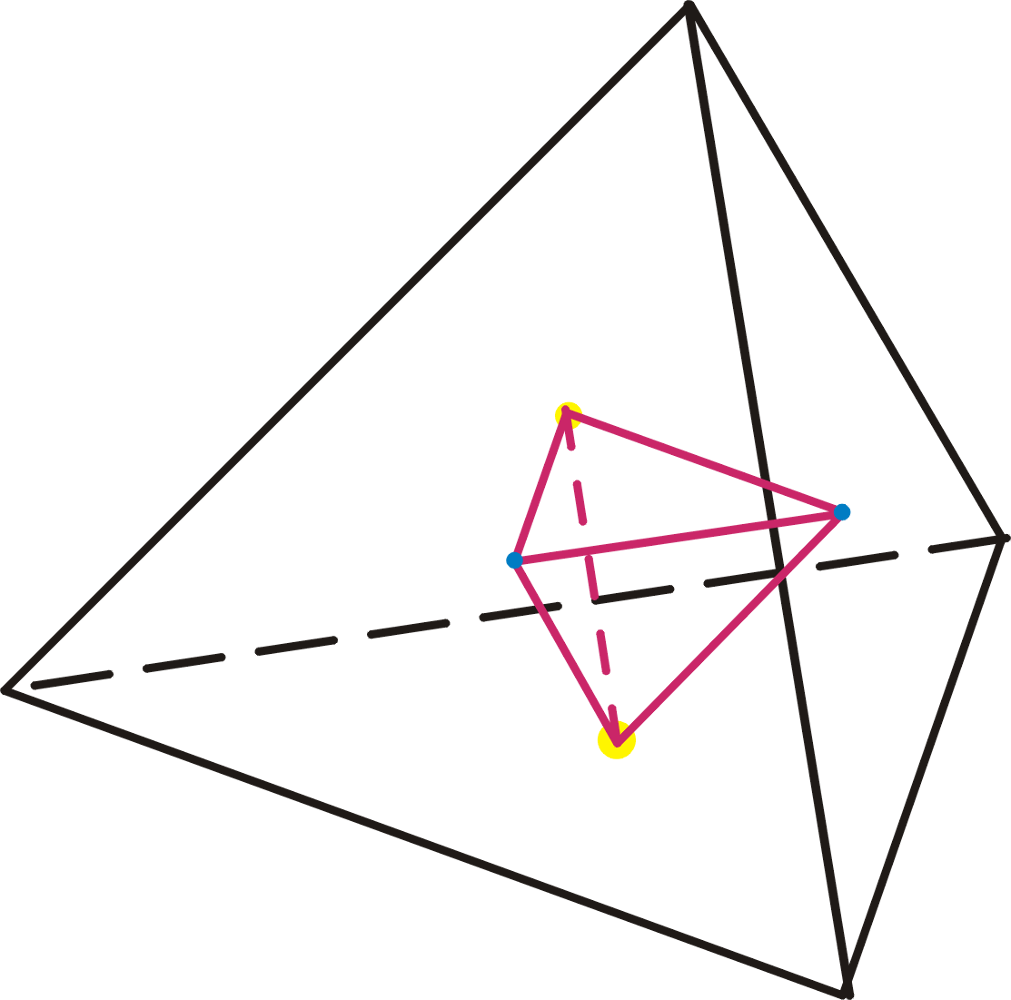
\includegraphics[height=210px]{../Grafiken/Duality_Tetra-Tetra.png} \\
 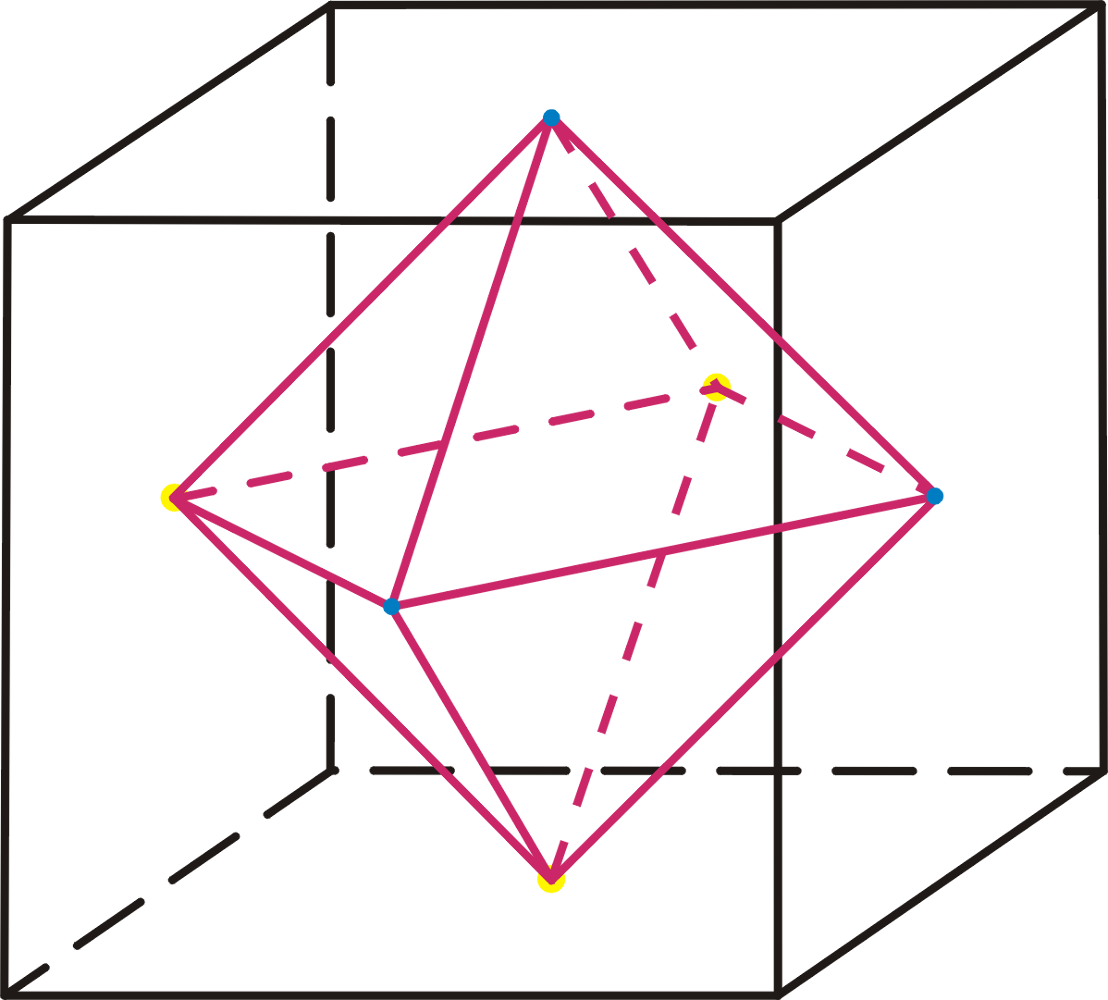
\includegraphics[height=210px]{../Grafiken/Duality_Hexa-Okta.png} \\
 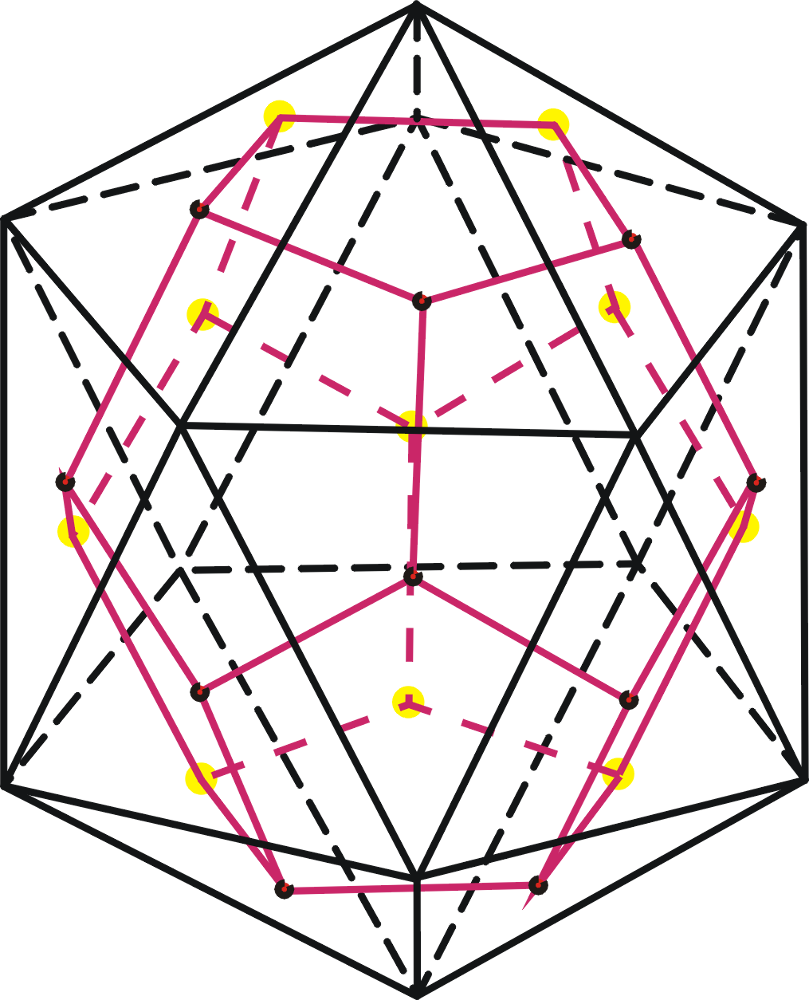
\includegraphics[height=210px]{../Grafiken/Duality_Iko-Dodek.png}
\end{center}
\end{document}
